%%%%%%%%%%%%%%%%%%%%%%%%%%%%%%%%%%%%%%%%%
% Beamer Presentation
% LaTeX Template
% Version 1.0 (10/11/12)
%
% This template has been downloaded from:
% http://www.LaTeXTemplates.com
%
% License:
% CC BY-NC-SA 3.0 (http://creativecommons.org/licenses/by-nc-sa/3.0/)
%
%%%%%%%%%%%%%%%%%%%%%%%%%%%%%%%%%%%%%%%%%

%----------------------------------------------------------------------------------------
%	PACKAGES AND THEMES
%----------------------------------------------------------------------------------------

\documentclass{beamer}

\mode<presentation> {

%\usetheme{default}
%\usetheme{Antibes}
%\usetheme{Boadilla}
\usetheme{JuanLesPins}
%\usetheme{Madrid}
%\usetheme{Rochester}



% As well as themes, the Beamer class has a number of color themes
% for any slide theme. Uncomment each of these in turn to see how it
% changes the colors of your current slide theme.

%\usecolortheme{beaver}
%\usecolortheme{dolphin}
%\usecolortheme{orchid}
%\usecolortheme{rose}
%\usecolortheme{seagull}
%\usecolortheme{seahorse}
%\usecolortheme{whale}
%\usecolortheme{wolverine}

%\setbeamertemplate{footline} % To remove the footer line in all slides uncomment this line
%\setbeamertemplate{footline}[page number] % To replace the footer line in all slides with a simple slide count uncomment this line

%\setbeamertemplate{navigation symbols}{} % To remove the navigation symbols from the bottom of all slides uncomment this line

\setbeamertemplate{caption}[numbered]
}

\usepackage{graphicx}
\usepackage{booktabs}
\usepackage{subfig}
\usepackage[%
	autocite    = superscript,
	backend     = bibtex,
	sortcites   = true,
	style       = numeric,
]{biblatex}
\addbibresource{reference.bib}

%----------------------------------------------------------------------------------------
%	TITLE PAGE
%----------------------------------------------------------------------------------------

\title[High speed Flight]{Learning High-Speed Flight in the Wild \autocite{high-speed-flight}}
\author{Edwin Jose George}
\institute[GCEK]{
	Guided by Dr. Rafeeque P C \\
	\medskip
	Department of Computer Science and Engineering \\
	Government College of Engineering Kannur
}
\date{\today}

\begin{document}

\begin{frame}
	\titlepage
\end{frame}

\begin{frame}{Overview}
	\tableofcontents
\end{frame}

%----------------------------------------------------------------------------------------
%	PRESENTATION SLIDES
%----------------------------------------------------------------------------------------
\section{Introduction}
\begin{frame}{Quad-drones}
	\begin{itemize}
		\item They are the most agile and dynamic machines, traversing extremely complex environments at high speeds. 
		\item This ability has led to their application in fields such as search and rescue, logistics, security, infrastructure, entertainment, and agriculture.
		\item To date, only expert human pilots have been able to fully exploit their capabilities. 
		\item Training of expert piolts - time consuming and costly
		\item The limiting factor for autonomous agile flight in arbitrary unknown environments is the coupling of fast and robust perception with effective planning. 
	\end{itemize}
\end{frame}

\begin{frame}{State of the art}
	\begin{itemize}
		\item Autonomous operation with onboard sensing and computation has been limited to low speeds. 
		\item Separate the navigation problem into subtasks: sensing, mapping, and planning. \\
		This approach has proven successful at low speeds
		\item The sub tasks are executed sequentially, leading to increased processing latency and compounding of errors through the pipeline.
		\item These issues can be mitigated to some degree by careful hand-tuning and engineering.
	\end{itemize}
\end{frame}

\begin{frame}{Proposed Solution}
	\begin{itemize}
		\item Here we propose an end-to-end approach that can autonomously fly quad rotors through complex natural and human-made environments at high speeds, with purely onboard sensing and computation.
		
		\item The key principle is to directly map noisy sensory observations to collision-free trajectories in a receding-horizon \autocite{receding_horizon} fashion. 
		
		\item This direct mapping drastically reduces processing latency and increases robustness to noisy and incomplete perception. 
		
		\item The sensorimotor mapping is performed by a convolutional network
	\end{itemize}
\end{frame}

\section{Constraints}
\begin{frame}{Constraints to meet}
	\begin{itemize}
		\item The perception system has to be robust to disturbances such as sensor noise, motion blur, and changing illumination conditions
		\item An effective planner is necessary to find a path that is both dynamically feasible and collision-free while relying only on noisy and partial observations of the environment.
		\item The limited computational resources that are available on board, make it difficult to achieve reliable perception and effective planning at low latency and high speeds.
		\item Other factors such as aerodynamics, torque, power, reaction delays etc.
	\end{itemize}
	The limiting factor for autonomous agile flight in arbitrary unknown environments is the \textbf{\textit{coupling of fast and robust perception with effective planning}}.
\end{frame}


\section{Model evolution}
\begin{frame}{State of the art Model}
	\begin{itemize}
		\item Some works tackle only perception and build high-quality maps from imperfect measurements. 
		\item Other works focus on planning without considering perception errors. 
		\item Numerous systems that combine online mapping with traditional planning algorithms have been proposed to achieve autonomous flight in previously unknown environments.
		\begin{itemize}
			\item 3d euclidean signed distance fields
			\item pushbroom stereo
			\item Rapid exploration
with multi-rotors
		\end{itemize} 
	\end{itemize}
\end{frame}

\begin{frame}{Traditional Methodology}
	\begin{itemize}
		\item The division of the navigation task into subtask
		\begin{itemize}
			\item Sensing
			\item Mapping
			\item Planning	
		\end{itemize} 
	
		\item Attractive from an engineering perspective because it enables parallel progress on each component and makes the overall system interpretable. 
		\item It leads to pipelines that largely neglect interactions between the different stages and thus compound errors. 
		\item Their sequential nature also introduces additional latency.
	\end{itemize}
\end{frame}

\begin{frame}{Recent Models}
	\begin{itemize}
		\item Proposal to learn end-to-end policies directly from data without explicit mapping and planning stages. 
		\item These policies are trained by imitating a human, from experience that was collected in simulation, or directly in the real world. More recent work has demonstrated that very agile control policies can be trained in simulation. 
		\item Policies produced by the last approach can successfully perform acrobatic maneuvers, but can only operate in unobstructed free space and are essentially blind to obstacles in the environment.
	\end{itemize}
\end{frame}

\begin{frame}{This works}
	\begin{itemize}
		\item Here we present an approach to fly a quad rotor at high speeds in a variety of environments with complex obstacle geometry while having access to only onboard sensing and computation. 
		\item By predicting navigation commands directly from sensor measurements, we decrease the latency between perception and action while simultaneously being robust to perception artifacts, such as motion blur, missing data, and sensor noise.
	\end{itemize}
	
\end{frame}

\begin{frame}{Taxonomy of existing approaches for drone navigation}
	\centering
	\begin{figure}
		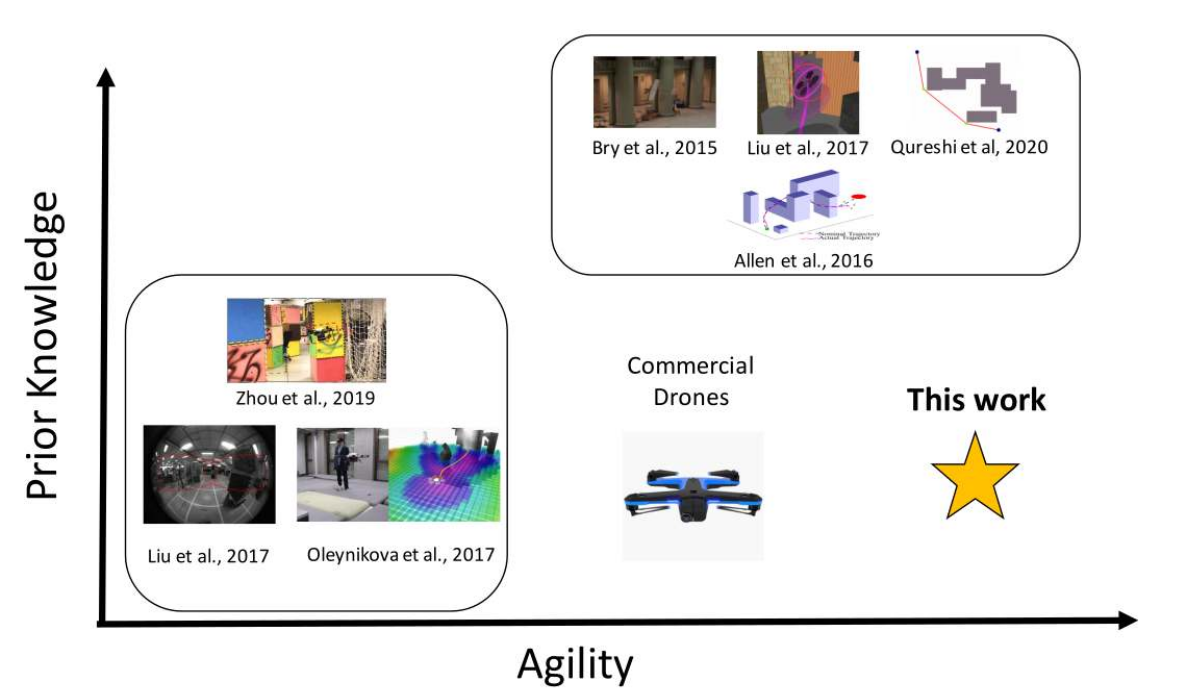
\includegraphics[height=2in]{images/taxonomy_navigation.png}
		\caption{Taxonomy of existing approaches for drone navigation in challenging and cluttered environments.}
	\end{figure}
\end{frame}

\section{Methodology}
\begin{frame}{Input (incomplete)}
	We leverage the abstraction of the input data to transfer the policy from simulation to reality. To this end, we utilize a stereo matching algorithm \autocite{stereoMatching} to provide depth images as input to the policy. 
\end{frame}


\begin{frame}{Navigation Policy (incomplete)}
	We train the navigation policy via privileged learning \autocite{Privileged_Learning} on demonstrations that are provided by a sampling-based expert. The existing global planning algorithms \autocite{global_planning} generally output a single trajectory, our expert uses Metropolis-Hastings \autocite{MH_hasting} sampling to compute a distribution of collision-free trajectories. We use our planner to compute trajectories with a short time horizon to ensure that they are predictable from onboard sensors and that the sampler remains computationally tractable. We bias the sampler toward obstacle-free regions by conditioning it on trajectories from a classic global planning algorithm [13].
	
\end{frame}

\begin{frame}{Neural Network Policy (incomplete)}
	We also reflect the multi-modal nature of the problem in the design and training of the neural network policy. Our policy takes a noisy depth image and inertial measurements as sensory inputs and produces a set of short-term trajectories together with an estimate of individual trajectory costs. The trajectories are represented as high-order polynomials to ensure dynamical feasibility. We train the policy using a multi-hypothesis winner-takes-all loss that adaptively maps the predicted trajectories to the best trajectories that have been found by the sampling-based expert. The policy network is designed to be extremely lightweight, which ensures that it can be executed on board the quadrotor at the update rates required for high-speed flight.
	
\end{frame}

\section{Result}

\subsection{Real-world environment}
\begin{frame}{Method of evaluation}
	'\begin{itemize}
		\item Results are confirmed in a variety of real-world environments using a \textit{custom-built physical quadrotor}
		\item Policy trained in simulation was deployed without any further adaptations.
		\item In all experiments, the drone was provided with a reference trajectory, which is not collision-free.
		\item The drone is tasked to follow that flight path and make adjustments as necessary to avoid obstacles.
		\item The performance is measured according to success rate
		\begin{itemize}
			\item The percentage of successful runs over the total number of runs
			\item A run successful if the drone reaches the goal location within a radius of 5 m without crashing.
		\end{itemize} 
	\end{itemize}
\end{frame}

\begin{frame}{Natural and Human-made environment}
	\begin{itemize}
		\item Natural Environment
		\begin{itemize}
			\item complex structure
			\item multiple options available to avoid obstacles. 
			\item A high-level understanding of the environment is necessary.
			\item Challenging illumination conditions
			\item Low texture surfaces (e.g. because of snow)
		\end{itemize}
	
		\item Human-made Environment
		\begin{itemize}
			\item Obstacles with a variety of sizes and shapes \\
			(e.g. a train, a crane, building and ruins)
			\item Limited number of flyable openings (eg. Narrow openings)
			\item Requires to initiate the avoidance maneuver well in advance.
		\end{itemize}
	\end{itemize}	
\end{frame}

\begin{frame}{Natural and Human-made environment - Graph }
	\begin{figure}
		\subfloat[Aggregate result]{
			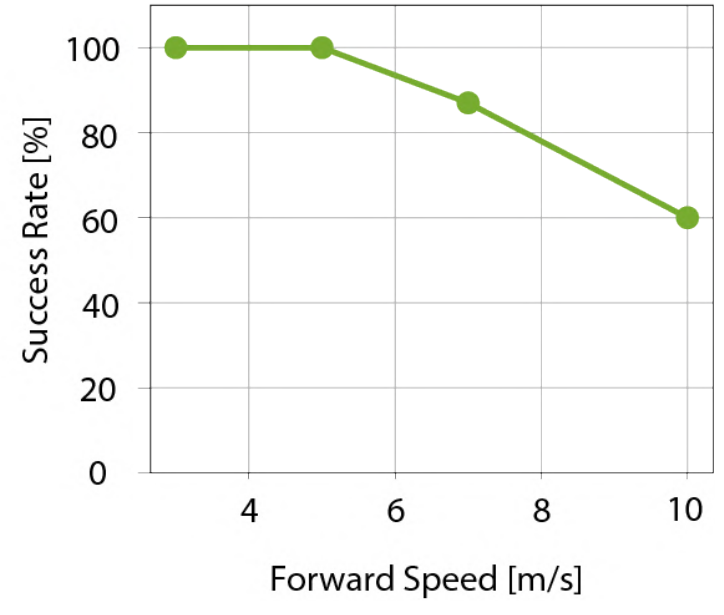
\includegraphics[width=1.5in]{images/natural-human-linegraph.png}
		}
		\subfloat[Individual result]{
			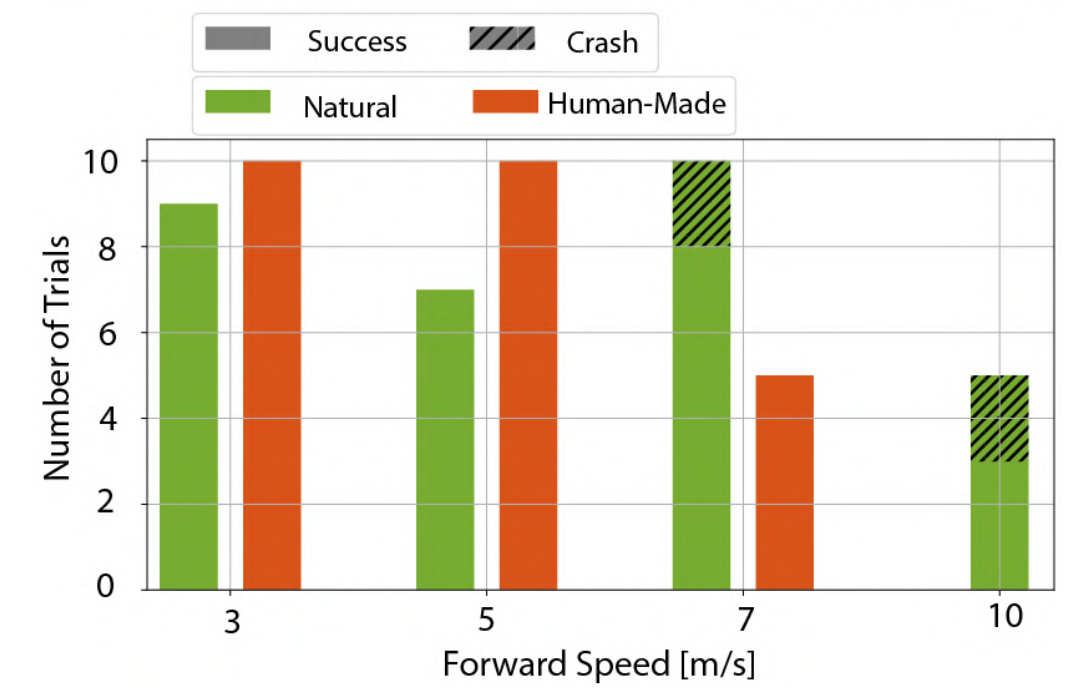
\includegraphics[width=2.5in]{images/natural-human-bargraph.png}
		}
		\caption{Trails on natural and human-made environment on physical drone}
	\end{figure}
\end{frame}

\subsection{Stimulated Environment}
\begin{frame}{Controlled Experiments - Comparative results}
	\begin{itemize}
		\item Two representative state-of-the-art approaches as selected as baselines for navigation in unknown environments: 
		\begin{itemize}
			\item Mapping and planning method - FastPlanner
			\begin{itemize}
				\item incrementally builds a map from a series of observations and plans a trajectory in this map to reach the
goal while avoiding obstacles.
			\end{itemize}
			\item Reactive planner
			\begin{itemize}
				\item uses instantaneous depth information to select the best trajectory from a set of pre-defined motion primitives
	based on a cost that encodes collision and progress toward the goal.
			\end{itemize}
		\end{itemize}
	
		\item All experiments are stimulated in the Flightmare simulator using the RotorS Gazebo plugin for accurate physics modeling and Unity as a rendering engine.
		
		\item The experiments are conducted in four different environments: a forest, a narrow gap, a disaster scenario, and a city street.
	
	\end{itemize}
\end{frame}

\begin{frame}{Controlled Experiments - Graphs}
	\begin{figure}
		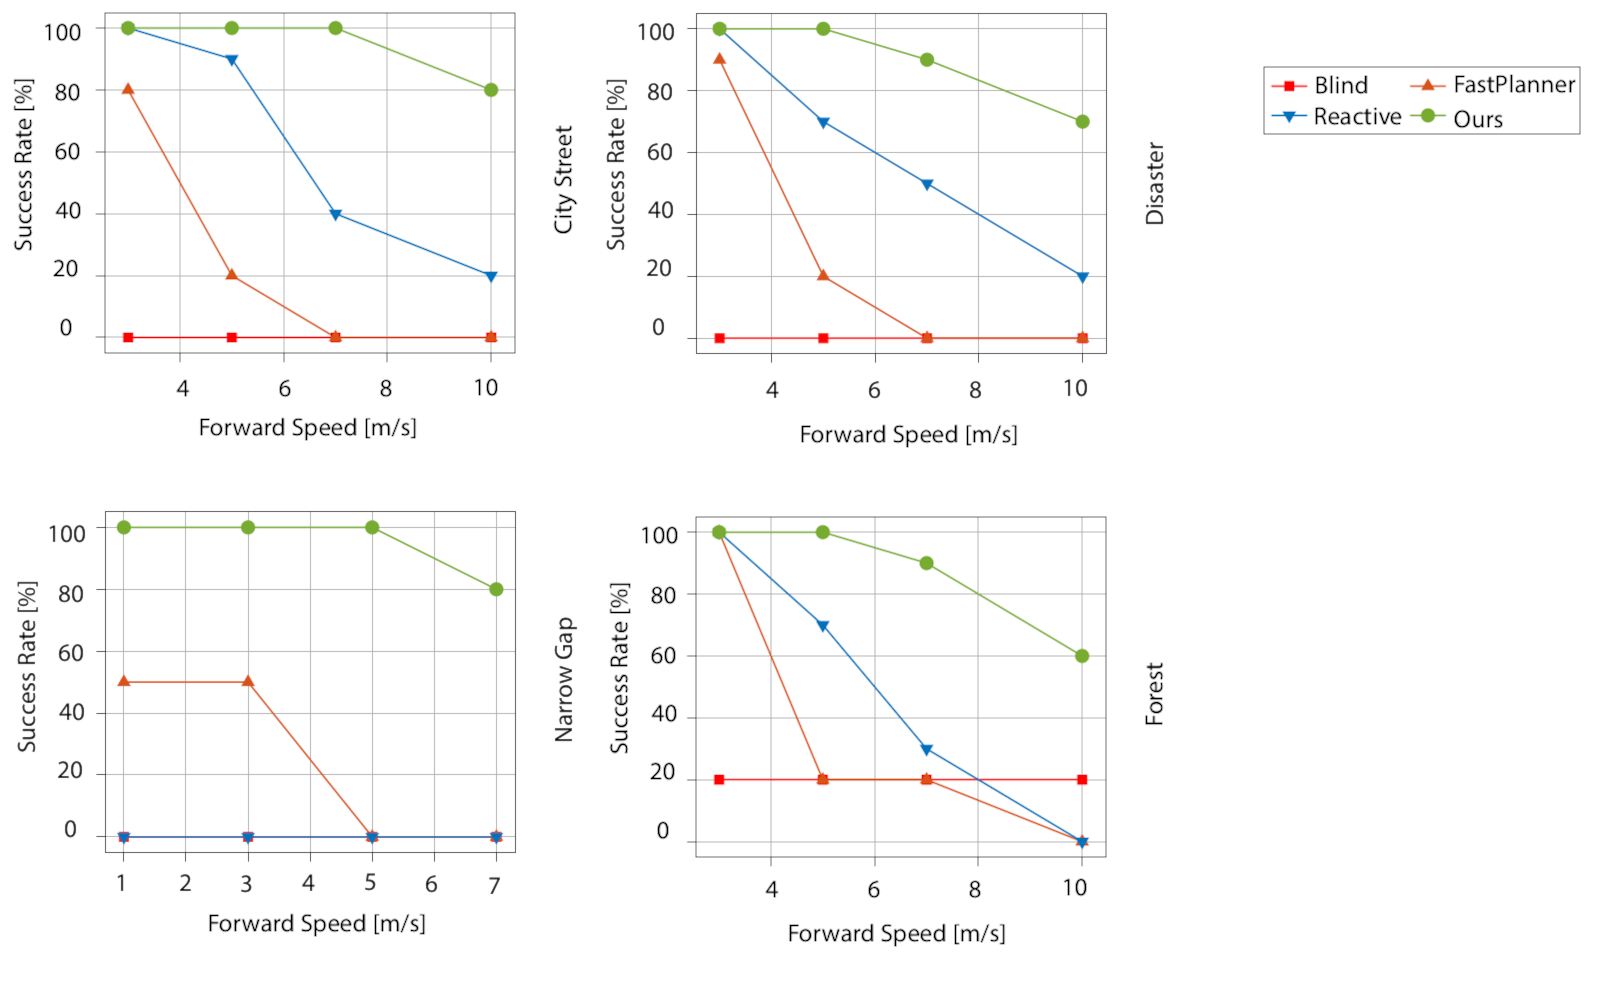
\includegraphics[width=4in]{images/controlled-experiments.png}
		\caption{Stimulated results}
	\end{figure}
	
\end{frame}

\begin{frame}[allowframebreaks]{The effect of latency and sensor noise}
	\begin{itemize}
		\item In this experiment, the quadrotor travels along a straight line at a constant forward speed and is required to laterally evade a single obstacle (a pole) while having only limited sensing range.
		\item The theoretical maximum speed is the speed at which the task is no longer feasible for each method. 
		\item The maximum speed depends on 
		\begin{itemize}
			\item sensing range - how far can an obstacle be accurately perceived
			\item latency of the visual sensor - the inverse of the frame rate
			\item processing latency - the time to convert an observation into motor commands.
		\end{itemize} 
	
		\pagebreak
		
		\begin{block}{Formula}
			theoretical maximum speed
			\begin{equation}
				v_{max} = \frac{s}{t_s + t_p + t_{rot} + \sqrt{\frac{2*r_{obs}}{sin(\theta)*c_{max}}}}
			\end{equation}
		\end{block}
		\item The experiment is run in two settings:
		\begin{itemize}
			\item with \textbf{ground-truth depth} information - to isolate the effect of latency on performance
			\item with \textbf{depth estimated by stereo matching}\autocite{stereoMatching} - to analyze the effect of sensing errors on performance.
		\end{itemize}
	\end{itemize}
\end{frame}

\begin{frame}{Effect of latency and noise - graphs}
	\begin{figure}
		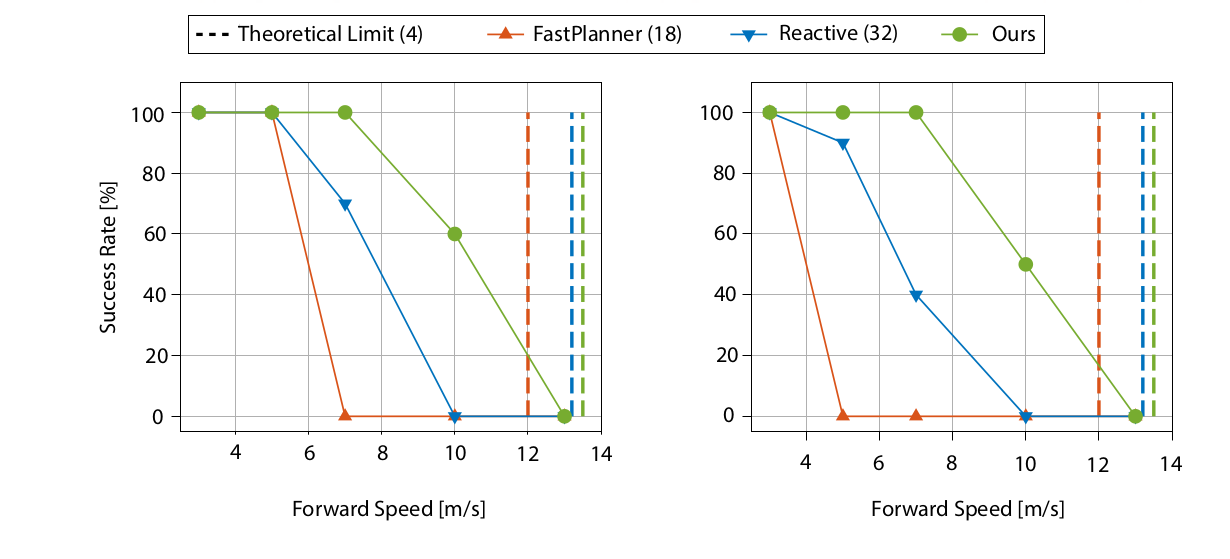
\includegraphics[width=4in]{images/noise-graph.png}
		\caption{The effect of sensor noise on performance. The experiment is performed on ground-truth-depth (1) and stereo-depth (2)}
	\end{figure}
\end{frame}

\begin{frame}{Effect of latency and noise - images}
	\begin{figure}
		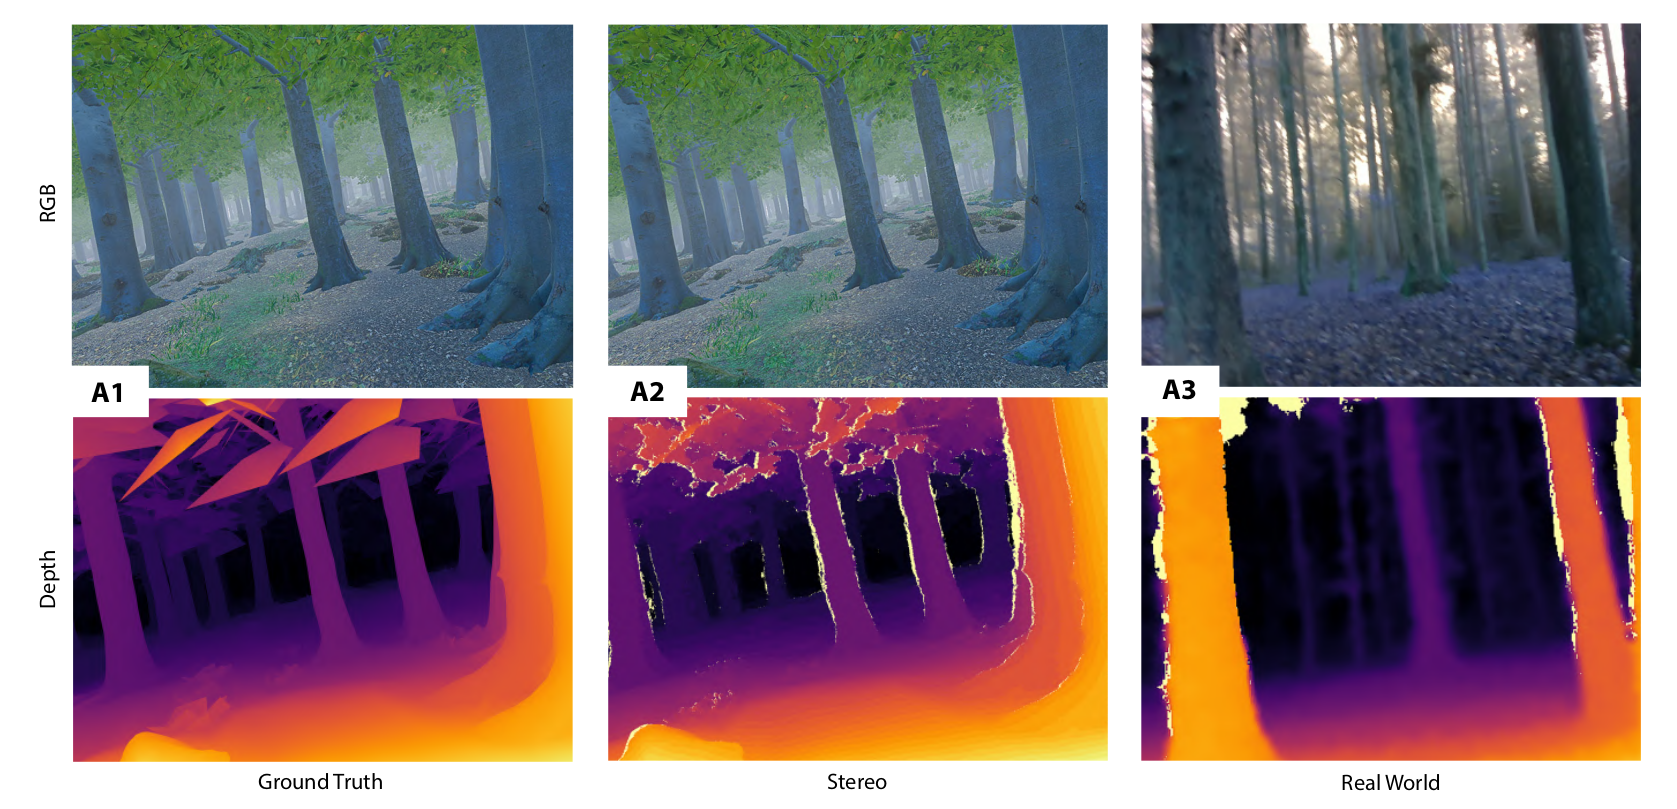
\includegraphics[width=4in]{images/stimulation and stereo.png}
		\caption{The image perceived by the system}
	\end{figure}
\end{frame}

\section{Conclusions}
\begin{frame}{Conclusion}
	\begin{itemize}
		\item We achieve high speed flight by training a neural network to imitate an expert with privileged information in simulation.
		
		\item To cope with the complexity of the task and to enable seamless transfer from simulation to reality, several technical contributions accounting multi-modality include
		\begin{itemize}
			\item sampling-based expert
			\item neural network architecture
			\item training procedure
		\end{itemize} 
		
		\item We use an abstract, but sufficiently rich input representation that considers real-world sensor noise.
	\end{itemize}
	The combination of these innovations enables the training of robust navigation policies in simulation that can be directly transferred to diverse real-world environments without any fine-tuning on real data.
	
\end{frame}

\section{Future Scope}
\begin{frame}[allowframebreaks]{Opportunities for future works}
	\begin{itemize}
		\item Low success rates at average speeds of 10 $m/s$ or higher in the real world. \\
		\textbf{Reason}: At higher speeds, feasible solutions require temporal consistency over a long time horizon and strong variations of the instantaneous flying speed.\\
		\textbf{Solution} : Engineering a more complex expert by specifically tailored heuristics to find approximate solutions. 
		
		\item Perception latency: Faster sensors can provide more information about the environment in a smaller amount of time. This could enable further reducing sensitivity to noise and promote a quicker understanding of the environment. 
		\textbf{Solution} : Use of event cameras, especially in the presence of dynamic obstacles.
		
		\item Mismatch between the simulated and physical drone in terms of dynamics and perception. \\
		\textbf{Reason} : aerodynamics effects, motor delays, and dropping battery voltage. \\
		\textbf{Solution} : Increasing the fidelity of the simulated drone and making the policy robust to the unavoidable model mismatches.
		
		
	\end{itemize}
	
\end{frame}

\section{References}
\begin{frame}[allowframebreaks]{References}
	\printbibliography
\end{frame}

\end{document}